%% LyX 2.4.4 created this file.  For more info, see https://www.lyx.org/.
%% Do not edit unless you really know what you are doing.
\documentclass[english,hebrew]{article}
\usepackage[HE8,T1]{fontenc}
\usepackage[utf8]{inputenc}
\usepackage{babel}
\usepackage{amssymb}
\usepackage{graphicx}
\usepackage[]
 {hyperref}

\makeatletter

%%%%%%%%%%%%%%%%%%%%%%%%%%%%%% LyX specific LaTeX commands.
%% A simple dot to overcome graphicx limitations
\newcommand{\lyxdot}{.}


\makeatother

\begin{document}
\title{על משחקי קלפים, פסי רכבת ונקודות באינסוף}
\maketitle
\begin{description}
\item [{קטגוריות:}] קומבינטוריקה
\item [{תגים:}] מישור פרוייקטיבי
\item [{מזהה:}] \L{dobble\_and\_projective\_planes}
\end{description}

\section{מבוא}

מדי פעם משחק שהוא מאוד מתמטי באופיו מצליח להפוך ללהיט בציבור הכללי,
והפעם אני רוצה לדבר על דאבל )\L{Dobble}, שנקרא גם \L{Spot It!} לפעמים(:

\L{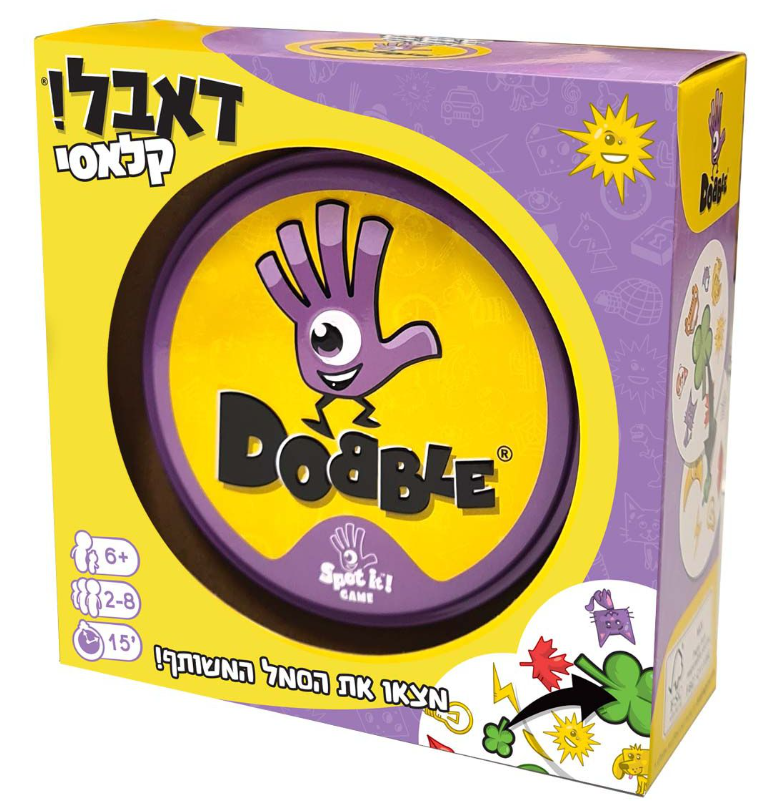
\includegraphics{../static/img/2026/Dobble1}}

יש כל מני דרכים לשחק את המשחק הזה, אבל הרעיון הבסיסי מאחורי כולן הוא
זה: המשחק כולל חבילת קלפים )עגולים(. על כל קלף יש {\beginL 8\endL}
ציורים של אובייקטים כלשהם )למשל: שעון, מרגנית, נורה, צב, עכביש וכו'(.
הקלפים בנויים איכשהו כך שתתקיים התכונה המופלאה הבאה: לכל זוג קלפים
שנבחר, יש להם \textbf{בדיוק} אובייקט משותף אחד. כל הוריאנטים של משחקי
דאבל מתבססים על האתגר הבא: בהינתן שני קלפים, מצאו כמה שיותר מהר את
האובייקט המשותף לשניהם.

\L{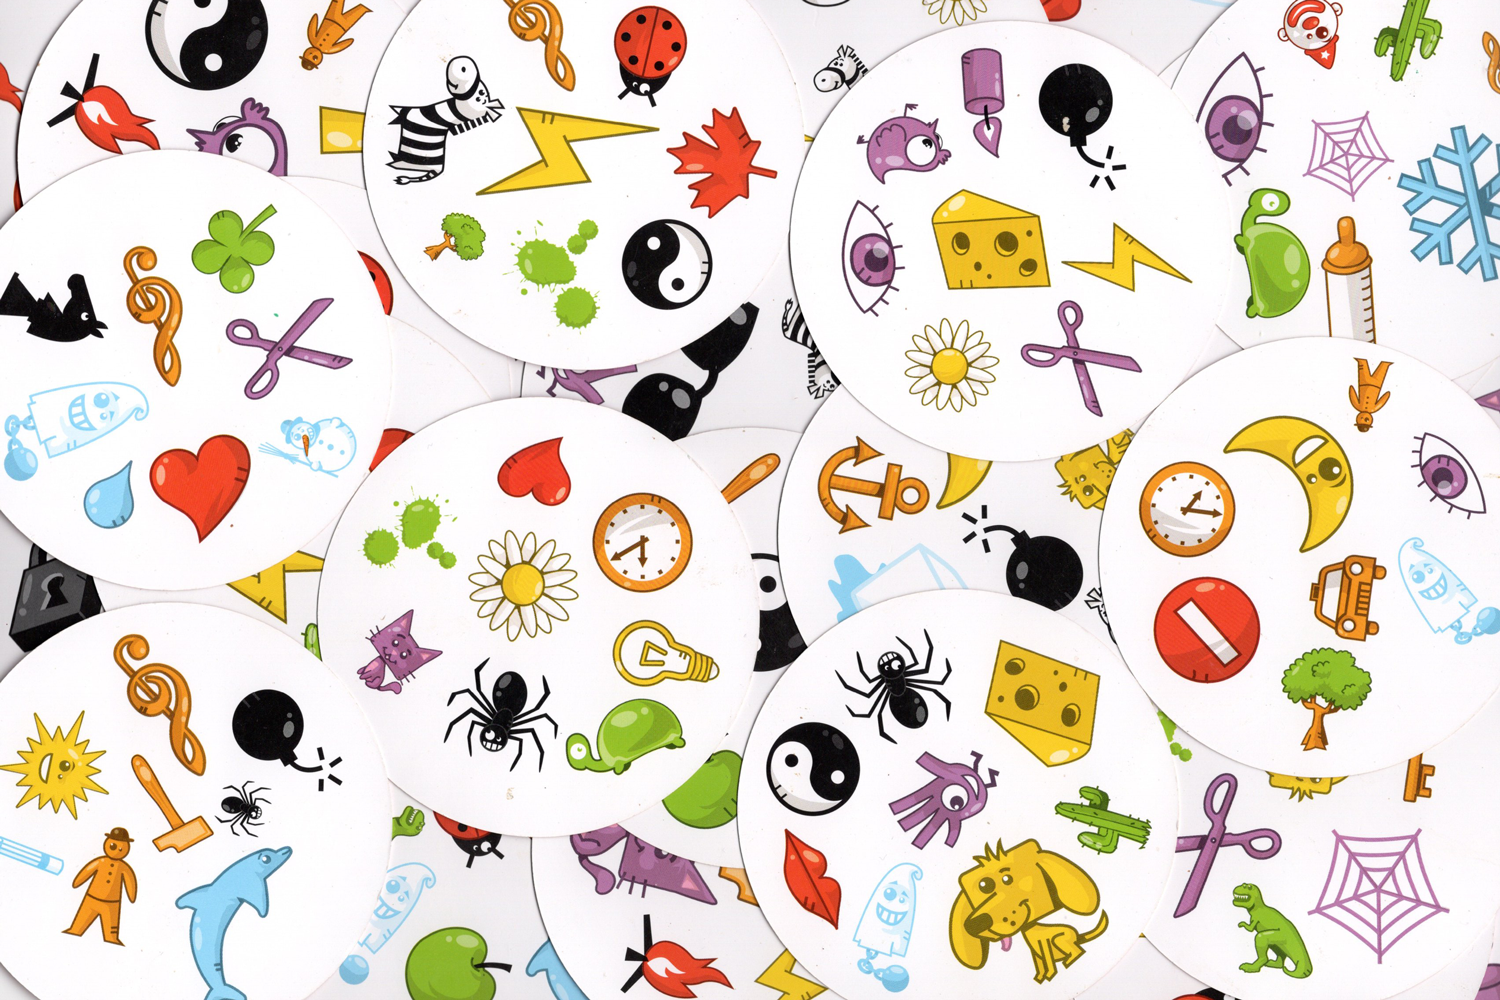
\includegraphics{../static/img/2026/Dobble2}}

יש במשחק הזה היבט לא מתמטי משמעותי מאוד - ההיבט של \textbf{עיצוב}
הקלפים, שהוא לדעתי בעל חלק חשוב בהצלחה של המשחק. החל בבחירה בקלפים
עגולים )מה שגורם לכך שכשמורידים קלף לשולחן, אוטומטית בוחרים באקראי
\textquotedblleft סיבוב\textquotedblright{} של האובייקטים שעליו( ,
עבור באיורים עצמם וכלה בטריק של גודל שונה לאותו אובייקט בין קלפים
שונים כדי להקשות על מציאת הצורה המשותפת. אבל מעבר להיבט הזה, יש גם
משהו חמוד מאוד בהיבט המתמטי שלו. שתי שאלות מתעוררות כמעט מייד: \textbf{למה}
בכלל אפשרי שתהיה סיטואציה כזו של חבילת קלפים גדולה שכל שני קלפים ממנה
חולקים \textbf{בדיוק} אובייקט אחד, ו\textbf{איך} מוצאים את החבילה
הזו? הרי אם סתם ננסה ליצור קלפים בעצמנו מהר מאוד נסתבך ממש. אם יצרנו
איכשהו {\beginL 10\endL} קלפים, אז הקלף ה-{\beginL 11\endL} יהיה חייב
להיות בעל אובייקט משותף עבור \textbf{כל} הקלפים שיצרנו עוד כה אבל
\textbf{אסור} שיהיו שני אובייקטים משותפים - אם ננסה ליצור את זה בניסוי
וטעייה יהיה מדובר בגיהנום. אז האם יש דרך אחרת?

באופן מרהיב, בהחלט יש דרך אחרת שלא כוללת ניסוי וטעיה. באופן עוד יותר
מרהיב, היא מתבססת על \textbf{גאומטריה} וספציפית על \textbf{גאומטריה
פרוייקטיבית} שהיא מה שמקבלים כאשר אנחנו מסתכלים על פסי רכבת ואומרים
לעצמנו \textquotedblleft המממ... אנחנו יודעין שפסי הרכבת הללו מקבילים
ולא ייפגשו לעולם אבל מאיפה שאנחנו עומדים זה נראה שהם הולכים להיפגש
\textbf{באינסוף}.\textquotedblright{}

\L{
\includegraphics{C:/Users/GADIALEKSANDROWICZ/Dropbox/Websites/new_blog/static/img/2026/Dobble3.jpg}}

בואו נדבר על זה.

\section{חלק ראשון, ובו אין לנו מושג מה אלו קווים ונקודות}

\textbf{קווים} זה מושג שמגיע מגאומטריה. כולנו מכירים גאומטריה אינטואיטיבית,
אבל מה זה בעצם אומר? מה שאנחנו רואים בבית הספר הוא מה שנקרא גאומטריה
\textbf{אוקלידית} שאפשר לחשוב עליה כך: יש לנו דף נייר. על הדף יש נקודות
וקווים. מה זו נקודה? נו, הדבר הזה שמקבלים כשלוחצים עם העפרון על הדף.
ומה זה קו? נו, הדבר הזה שמקבלים כשששמים סרגל ואז מצמידים אליו עיפרון
ומזיזים אותו קדימה-אחורה. אנחנו יודעים מה זה קווים ונקודות, כן? לא
צריך להסביר לנו.

אבל מה זה אומר, \textbf{פורמלית}, מתמטית? ובכן, הנה הסוד האפל של המתמטיקה:
כלום. זה אומר כלום. שום דבר. אין לנו במתמטיקה הסבר לשאלה \textquotedblleft מה
זו נקודה\textquotedblright{} ו\textquotedblright מה זה קו\textquotedblright{}
בגאומטריה.

אחרי שזעקות השוד ושבר לנוכח חשיפת הסוד האפל נרגעו, אפשר לצחוק על זה.
מה זאת אומרת אין הסבר. מה עם אוקלידס בעצמו? הרי הוא כתב ספר יפה, \textquotedblleft יסודות\textquotedblright ,
כולנו סובלים מהספר הזה עד היום. הוא מסביר שם בדיוק את הכל, למה שלא
נבדוק מה הוא אומר?

ובכן, אוקלידס כתב ביוונית שאני לא מבין אז אני לא אביא אותה כאן, אבל
אפשר למצוא תרגומים בשלל מקומות כולל באינטרנט. \href{http://aleph0.clarku.edu/~djoyce/java/elements/elements.html}{כאן}
למשל יש תרגום לאנגלית שהכין \L{David E. Joyce}. \href{https://hebrewscience.org/}{וכאן}
יש משהו קסום - תרגום לעברית מהמאה ה-{\beginL 13\endL} של ר’ יעקב בן
מכיר. בואו נראה איך, על פי שני התרגומים הללו, אוקלידס מגדיר \textquotedblleft נקודה\textquotedblright :
\begin{itemize}
\item \textquotedblleft הנקודה היא דבר אין חלק לה. \textquotedblleft{}
\item \textquotedblleft\L{A point is that which has no part.}\textquotedblright{}
\end{itemize}
זה... מעליב. זה לא אומר מה נקודה היא \textbf{כן}, אלא מה היא \textbf{לא}
- היא לא משהו שמורכב מדברים יותר בסיסיים. אבל נו, שיהיה, חייבים להתחיל
מ\textbf{משהו} שלא יוגדר בעזרת דברים פשוטים יותר. אז עכשיו שיש לנו
נקודה בטח נוכל להגדיר קו בתור \textquotedblleft המון נקודות ביחד\textquotedblright{}
בצורה כלשהי, לא? אז זהו, שלא:
\begin{itemize}
\item \textquotedblleft והקו הוא אורך אין רוחב לו.\textquotedblright{}
\item \textquotedblleft\L{A line is breadthless length.}\textquotedblright{}
\end{itemize}
כאן יש משהו על דרך החיוב - לקו יש \textquotedblleft אורך\textquotedblright{}
)לא ברור מה זה אורך( אבל גם שלילה: אין לו \textquotedblleft רוחב\textquotedblright{}
)לא ברור מה זה רוחב(. שימו לב מה אין פה: לא אומרים שקו מורכב מנקודות;
לא אומרים שהוא ישר; לא אומרים אם הוא בעל קצוות או מתמשך עד לאינסוף.

עכשיו, כמובן שההגדרות הללו מתאימות יפה מאוד לאינטואיציה שיש לנו ממה
שקורה עם דף ועפרון. נקודה היא - אה, נקודתית? אפשר לחשוב עליה בתור
דבר בסיסי שכזה. קו הוא, ובכן, ארוך, אבל זזים בו רק \textquotedblleft בכיוון
אחד\textquotedblright{} ולכן אין לו רוחב כמו נאמר למלבן. מה שקורה פה
הוא שהדברים שאנחנו עושים על נייר עם עיפרון הם פרשנות אפשרית אחת של
הגאומטריה )או ליתר דיוק, גרסה אידאלית של מה שאנחנו עושים על נייר,
שבה באמת אין לנקודה גודל ולקו אין רוחב( אבל יש עוד פרשנויות אפשריות,
והיופי בגאומטריה הוא שהיא מדברת על \textbf{כל} הפרשנויות הללו בבת
אחת. את זה כל אני אומר בתור הכנה לכך שמה שנתעסק בו בפוסט הזה יהיה
פרשנות אחרת, לא כל כך שונה אבל גם לא כל כך דומה למה שאנחנו מכירים.

עכשיו, אם נקודה וקו הם מושגים לא מוגדרים, איך בכלל אפשר לעשות איתם
משהו? בשביל זה אוקלידס מציג \textbf{אקסיומות} שהן מעין הנחות בסיס
על טיב היחסים והאינטראקציות בין האובייקטים הללו. לפני כן הוא מציג
עוד שלל הגדרות שפחות קריטיות לנו, למשל מה זו זווית ומה זה מעגל, ואז
הוא מגיע אל חמש האקסיומות שלו, שאנסח בלשון מודרנית ולא בלשון של אוקלידס:
\begin{enumerate}
\item אפשר למתוח קו ישר בין כל שתי נקודות.
\item ניתן להמשיך קו ישר ללא הגבלה.
\item בהינתן שתי נקודות אפשר לבנות מעגל שאחת הנקודות היא מרכזו והקו שמחבר
את הנקודות הוא הרדיוס שלו.
\item כל הזוויות הישרות שוות זו לזו.
\item דרך נקודה מחוץ לישר ניתן להעביר ישר יחיד שמקביל לישר הנתון.
\end{enumerate}
אקסיומות {\beginL 3-4\endL} לא יהיו רלוונטיות לנו הפעם. באקסיומות
{\beginL 1-2\endL} מופיע \textquotedblleft קו ישר\textquotedblright{}
שלא ברור מה הוא - אוקלידס מגדיר אותו קודם אבל בהגדרה חסרת פשר למדי.
עדיין, יש לנו את האינטואיציה להסתמך עליה, ואפשר להבין את האקסיומות
הללו בתור הצהרת כוונות: קו ישר זה משהו שיכול לגעת בנקודות, כלומר לכל
זוג של קו ונקודה מתקיים ביניהם היחס \textquotedblleft נוגעים/לא נוגעים\textquotedblright .
זו האינטראקציה המהותית בין שני המושגים המרכזיים הללו. אקסיומה {\beginL 2\endL}
גם מאפשרת לנו לחשוב על קווים בתור משהו שהוא לא תחום במרחב אלא \textquotedblleft הולך
עד לאינסוף\textquotedblright{} )למרות שזה לא נאמר פה במפורש(.

אקסיומה {\beginL 5\endL} היא מעניינת מאוד. הניסוח המקורי שלה שונה
למדי, אבל שקול לזה שהבאתי פה, שהוא הניסוח המודרני המקובל. בניסוח המקורי
המילה \textquotedblleft מקביל\textquotedblright{} לא מופיעה בה, אבל
זה לא נורא כי אוקלידס הגדיר \textquotedblleft ישרים מקבילים\textquotedblright{}
במפורש קודם: אלו שני קווים ישרים שלא משנה כמה נמשיך אותם, הם \textbf{לעולם
לא ייפגשו}. אקסיומת המקבילים בפרט אומרת שקווים מקבילים \textbf{קיימים}:
לכל קו ישר שניקח, יש קווים שמקבילים לו. לא סתם יש קווים שמקבילים לו,
תבחרו נקודה שרירותית בעולם - עדיין תוכלו למצוא ישר שמקביל לו גם עם
האילוץ הנוסף שהוא צריך לעבור דרך הנקודה הזו. במילים אחרות, יש \textbf{המון}
מקבילים לקו ישר.

בגאומטריה פרוייקטיבית הדבר הזה הולך לפח. הרעיון המהותי של גאומטריה
פרוייקטיבית, שמגיע בדיוק מאותו ציור פסי רכבת שראינו קודם, הוא שישרים
מקבילים לא הולכים להתקיים, כי גם לישרים ש\textquotedblright נראים
מקבילים\textquotedblright{} במובן של הגאומטריה האוקלידית תהיה נקודה
שבה הם ייפגשו - ב\textquotedblright אינסוף\textquotedblright{} )שכזכור
אמרנו בנפנוף ידיים מופרע שאפשר להמשיך ישרים עד אליו(.

נשמע כמו נפנוף ידיים מזעזע? בדיוק בשביל זה יש לנו את הגישה האקסיומטית,
שכבר ראינו שהיא הבסיס האמיתי גם של הגאומטריה שאנחנו רגילים אליה. נתחיל
עם להציג אקסיומות לגאומטריה פרוייקטיבית, נראה דברים שמתאימים להן,
ופתאום ה\textquotedblright נפגשים באינסוף\textquotedblright{} הזה לא
ייראה מופרך כל כך. על הדרך גם נפגוש את הקלפים של דאבל.

מה שאני הולך להגדיר נקרא \textbf{מישור פרוייקטיבי}. במישור פרוייקטיבי
יש שני סוגים של אובייקטים: נקודות וישרים. גם פה, אין שום נסיון להגיד
מי האובייקטים הללו אם איך הם נראים - רק חשוב הקשר שיש ביניהם. עכשיו,
טבעי לנו להגיד ש\textquotedblright נקודה נמצאת על ישר\textquotedblright ,
אבל יש בעיה עם הניסוח הזה כי הוא \textbf{לא סימטרי} - הוא רומז מילולית
שישרים מורכבים מנקודות, בעוד שנקודות כמובן אינן מורכבות מקווים. אנחנו
רוצים לנטרל את ההטיות הלשוניות הללו אז נשתמש במילה נייטרלית יותר -
\textbf{חילה} )\L{incidence}(. נקודה וישר יכולים לחול זו בזה )אבל
לא ישר בישר או נקודה בנקודה(. עכשיו אפשר לנסח בקלות את האקסיומות:
\begin{enumerate}
\item לכל שתי נקודות שונות זו מזו, קיים ישר \textbf{יחיד} שחל בשתיהן.
\item לכל שני ישרים שונים זה מזה, קיימת נקודה \textbf{יחידה} שחלה בשניהם
)בפרט, מכאן נובע שאין ישרים מקבילים(.
\item קיימות ארבע נקודות כך שאין ישר שחל על יותר משתיים מהן.
\end{enumerate}
שימו לב למשהו מעניין באקסיומות הללו - הן כמעט סימטריות: {\beginL 1\endL}
ו-{\beginL 2\endL} הן אותו הדבר בהחלפת התפקיד של ישר ונקודה. לעומת
זאת {\beginL 3\endL} היא לא סימטרית \textbf{אבל} אפשר להוכיח מתוך
שלוש האקסיומות הללו גם את הגרסה ה\textquotedblright דואלית\textquotedblright{}
שלה: שקיימים ארבעה ישרים כך שאין נקודה שחלה על יותר משניים מהם. הדואליות
הזו היא עיקרון כללי - לכל טענה שנכונה על מישור פרוייקטיבי סופי ניתן
להפוך את התפקידים של \textquotedblleft ישרים\textquotedblright{} ו\textquotedblright נקודות\textquotedblright{}
ולקבל עוד טענה נכונה.

ובכן, אלו האקסיומות, אבל אקסיומות הן בסך הכל אוסף סימבולים חסר פשר
שלא מבינים מה הוא רוצה מהחיים שלנו כל עוד אנחנו לא רואים בעיניים דוגמאות
למשהו שמקיים אותן. בגאומטריה אוקלידית יש לנו משהו כזה - דף נייר עם
עפרון. אנחנו צריכים להתחיל עם דוגמאות כאלו גם עבור מישורים פרוייקטיביים.

\section{חלק שני, שבו יש לנו מושג מה זה המישור של פאנו והקלפים של דאבל אבל
לא הרבה יותר מכך}

הדוגמא הפשוטה ביותר שאני מכיר למישור פרוייקטיבי נקראת \textbf{המישור
של פאנו} ונראית ככה:

\L{
\includegraphics{C:/Users/GADIALEKSANDROWICZ/Dropbox/Websites/new_blog/static/img/2026/Fano_plane.svg.png}}

מה יש לנו פה? זה ציור שבא להמחיש סיטואציה שבה יש לנו שבע נקודות ושבעה
ישרים. הנקודות הן העיגולים השחורים הקטנים; הישרים הם הקווים שבאיור,
כולל הקו שהוא בכלל מעגל. זה נשמע מוזר כי המילה \textquotedblleft ישר\textquotedblright{}
עלולה לעורר בנו ציפייה שאם מציירים ישרים הם יראו כמו, ובכן, ישרים
- אבל זכרו, כל מה שיש לנו הוא את האקסיומות והן לא דורשות שום דבר כזה.
גם הציור הוא בסך הכל ציור. היה אפשר לצייר את אותו דבר בדרכים אחרות.
היה אפשר גם להגיד שהמישור מורכב מקבוצת הנקודות \L{$\left\{ p_{1},p_{2},p_{3},p_{4},p_{5},p_{6},p_{7}\right\} $}
וקבוצת הישרים \L{$\left\{ l_{1},l_{2},l_{3},l_{4},l_{5},l_{6},l_{7}\right\} $}
כך שלמשל הישר \L{$l_{3}$} חל עם הנקודות \L{$p_{2},p_{5},p_{7}$}.
אבל דרך תיאור כזו היא כמובן הרבה יותר מסורבלת מאשר האיור הנחמד שלמעלה
ואין בה יותר אינפורמציה מאשר יש בו, ולכן אנחנו משתמשים בו.

באיור הזה קל לראות בעיניים שכל ישר חל בדיוק עם שלוש נקודות, וכל נקודה
חלה בדיוק עם שלושה ישרים. קל לראות שאקסיומות {\beginL 1\endL} ו-{\beginL 2\endL}
מתקיימות. בשביל אקסיומה {\beginL 3\endL} צריך לעבוד טיפ-טיפה יותר:
אם ניקח סתם ארבע נקודות, בהחלט ייתכן ששלוש מהן יהיו על אותו ישר, למשל
אם ניקח את שלוש הנקודות התחתונות. אבל בואו ניקח את כל שלוש הנקודות
שהן הקודקודים של ה\textquotedblright משולש\textquotedblright{} - בבירור
אין ישר שעובר דרך שלושתן. עכשיו נוסיף אליהן את נקודת האמצע, שלא הייתה
על אף ישר שעבר דרך זוגות של שלושת הקודקודים הללו - קיבלנו קבוצה של
ארבע נקודות כך שאין ישר שחל על יותר משתיים מהן, כך שהאקסיומות מתקיימות
- הדבר הזה הוא מישור פרוייקטיבי!

זה די שונה מהאינטואיציה הגאומטרית הרגילה שלנו, כי אנחנו חושבים על
מישור בתור משהו שמכיל\textbf{ אינסוף }נקודות )כי למשל בואו נמתח קו
בין הנקודות {\beginL 0\endL} ו-{\beginL 1\endL}; באמצע הקו יש את הנקודה
\L{$\frac{1}{2}$}, ובאמצע הקו בין {\beginL 0\endL} ו-\L{$\frac{1}{2}$}
יש את הנקודה \L{$\frac{1}{4}$} וכן הלאה עד אינסוף(. כאן לעומת זאת
יש לנו מישור פרוייקטיבי \textbf{סופי} - אבל שוב, כל מה שאנחנו משתמשים
בו כדי לבדוק אם משהו הוא מישור פרוייקטיבי הוא האקסיומות, והן בוודאי
לא דורשות אינסופיות.

איך זה קשור לדאבל? פשוט מאוד: תחשבו על הנקודות בתור \textbf{אובייקטים}
ועל הישרים בתור \textbf{קלפים}. מה שהמישור של פאנו נותן לנו הוא מן
גרסה פשוטה של דאבל: יש לנו {\beginL 7\endL} קלפים, ובסך הכל {\beginL 7\endL}
אובייקטים. על כל קלף יש {\beginL 3\endL} אובייקטים )וכל אובייקט מופיע
בדיוק ב-{\beginL 3\endL} קלפים( ולכל זוג קלפים יש בדיוק אובייקט אחד
שנמצא בשניהם יחד - זו \textbf{בדיוק} האקסיומה מס' {\beginL 2\endL},
\textquotedblleft לכל שני ישרים שונים זה מזה, קיימת נקודה \textbf{יחידה}
שחלה בשניהם.\textquotedblright{}

העניין הוא שבדאבל יש יותר קלפים, יותר אובייקטיבים והכי חשוב - יותר
אובייקטים שמופיעים על כל קלף - {\beginL 8\endL}, להבדיל מה-{\beginL 3\endL}
של המישור של פאנו. אז מה ההכללות של המישור של פאנו שנותנות את דאבל?

ובכן, זו שאלה די מעניינת.

ראשית, תוצאה שאני לא אוכיח כאן אבל היא לא \textbf{עד כדי כך} קשה להוכחה
מתוך האקסיומות מראה שאם יש לנו מישור פרוייקטיבי סופי, אז מספר הנקודות
שחלות עם כל ישר הוא זהה. מתבקש לסמן את המספר הזה באות כלשהי, אבל מתברר
שהכל יהיה פשוט יותר אם נשתמש באות כדי לתאר מספר שקטן ממנו ב-{\beginL 1\endL}.
כלומר, ניקח את האות \L{$N$} ומספר הנקודות שחלות עם כל ישר יהיה \L{$N+1$}.
המספר \L{$N$} עצמו נקרא \textbf{הסדר} של המישור הפרוייקטיבי, ותוצאה
שאפשר להוכיח מאוד בקלות היא שאם יש לנו מישור פרוייקטיבי מסדר \L{$N$}
אז יש בו בדיוק \L{$N^{2}+N+1$} נקודות )ובגלל הדואליות בין נקודות
וישרים, יש במישור הזה גם \L{$N^{2}+N+1$} ישרים(. ההוכחה של זה דורשת
סדרה של טענות עזר מעניינות בפני עצמן שדורשות רק את שלוש האקסיומות,
וזו הזדמנות מעולה לראות אקסיומות בפעולה. אבל - אני אחכה עם זה לחלק
האחרון של הפוסט. בינתיים בואו נסגור את הסיפור של דאבל.

אם כן, מה שראינו עד כה הוא שיש מספרי נקודות שעבורן פשוט לא יכול להתקיים
מישור פרוייקטיבי. אם נציב \L{$N=2,3,4,\ldots$} נקבל ב-\L{$N^{2}+N+1$}
את סדרת הערכים \L{$7,13,21,31,43,57,73,91,111,\ldots$}. כלומר, פשוט
אין מישור פרוייקטיבי עם \L{$15$} נקודות כי המספר הזה לא מופיע ברשימה
הזו. אבל האם זה עובד בכיוון ההפוך? האם לכל מספר שמופיע ברשימה אכן
קיים מישור פרוייקטיבי שזו כמות הנקודות שלו? ובכן, לא. עבור \L{$N=6$}
אנחנו מקבלים \L{$43$} ופשוט לא קיים מישור פרוייקטיבי עם {\beginL 43\endL}
נקודות. זו הדוגמא הראשונה לסיטואציה שבה הנוסחה \textquotedblleft נשברת\textquotedblright .

עבור \L{$N=7$}, לעומת זאת, בהחלט \textbf{קיים} מישור פרוייקטיבי בן
{\beginL 57\endL} נקודות )וגם בן {\beginL 57\endL} ישרים, כי עקרון
הדואליות(. עכשיו, זוכרים את המשמעות של \L{$N$}? \L{$N+1$} הוא מספר
הנקודות שיש על כל ישר, כלומר במישור הפרוייקטיבי הזה יש {\beginL 8\endL}
נקודות על כל ישר . נשמע מוכר? בוודאי, זה מספר האובייקטים שיש על קלף
של דאבל. במילים אחרות - הקלפים של דאבל הם בסך הכל הישרים של מישור
פרויקטיבי סופי מסדר \L{$7$}, ויש {\beginL 57\endL} קלפים כאלו.

רק מה, \textbf{אין} {\beginL 57\endL} קלפים של דאבל. בחבילת דאבל יש
רק {\beginL 55\endL} קלפים. מה זה, למה? אין לי שום הסבר, בוודאי לא
הסבר מתמטי. זו החלטה עיצובית של המשחק שנקשרו אליה כל מני צ'יזבטים
כמו זה שמכונות סטנדרטיות ליצירת קלפי משחק מותאמות ליצירה של חבילות
של {\beginL 55\endL} קלפים ){\beginL 52\endL} הקלפים הרגילים + {\beginL 2\endL}
ג'וקרים + קלף פרסומי אחד(. זה נשמע לי כמו צ'יזבט מוחלט )קלפי דאבל
בכלל לא דומים לקלפי משחק רגילים( ואין לי הסבר למה הלכו על {\beginL 55\endL}
ולא {\beginL 57\endL}, אבל אני לא חושב שיש פה סיבה מתמטית. כמובן,
אין בעיה עם זה שהסירו קלפים מהחבילה - המשחק לא דורש את \textbf{כל}
הקלפים, רק את הכלל של \textquotedblleft לכל שני קלפים יש אובייקט משותף
יחיד\textquotedblright{} המוכרת כעת בתור אקסיומה {\beginL 2\endL} של
מישור פרוייקטיבי.

אם כן, כשהחבר'ה של דאבל באו ליצור אותו הם לא היו צריכים לבצע שום עבודה
אלגוריתמית כי המתמטיקאים עשו אותה מזמן - המישור הפרוייקטיבי מסדר {\beginL 7\endL}
הוא משהו מוכר וידוע היטב. אבל, כמובן, זו לא תשובה טובה - לא אכפת לנו
שהמתמטיקאים מכירים את המישור הזה כבר מאה שנה, אנחנו רוצים להבין איך
\textbf{אנחנו} מסוגלים ליצור אותו, בעצמנו, יש מאין, מאפס.

והאמת, זה לא עד כדי כך מסובך. יש שיטה כללית. למעשה, לכל \L{$N$} שהוא
מהצורה \L{$N=p^{k}$} כאשר \L{$p$} הוא מספר \textbf{ראשוני} השיטה
הכללית הזו עובדת. יותר מכך - \textbf{כל} המישורים הפרוייקטיביים הסופיים
שהתגלו עד היום היו מסדר שהוא מהצורה \L{$p^{k}$}. הופס, עלינו על שאלה
פתוחה במתמטיקה! האם קיימים מרחבים פרוייקטיביים סופיים מסדר שאינו חזקה
של ראשוני? אנחנו לא יודעים, ומה שאנחנו כן יודעים הוא יחסית מעט. יש
תוצאה כללית מעניינת אחת, משפט \L{Bruck--Ryser--Chowla}: הוא אומר
שאם יש לנו מספר \L{$N$} ששקול ל-{\beginL 1\endL} או {\beginL 2\endL}
מודולו {\beginL 4\endL} )כלומר, \L{$N$} הוא מהצורה \L{$N=4k+1$}
או \L{$N=4k+2$}( אז \L{$N$} \textbf{לא יכול} להיות הסדר של מישור
פרוייקטיבי סופי אלא אם כן אפשר לכתוב את \L{$N$} בתור סכום של שני
ריבועים. למשל \L{$N=10$} הוא שקול ל-{\beginL 2\endL} מודולו {\beginL 4\endL}
ו\textbf{כן} אפשר לכתוב אותו בתור סכום של שני ריבועים, \L{$10=1^{2}+3^{2}$},
ולכן המשפט לא חל עליו; אבל \L{$6$} הוא {\beginL 2\endL} מודולו {\beginL 4\endL}
ואי אפשר לכתוב אותו כסכום של שני ריבועים ולכן המשפט מוכיח את הטענה
שאמרתי קודם - אין מישור פרוייקטיבי מסדר {\beginL 6\endL}, כלומר עם
{\beginL 43\endL} נקודות.

עכשיו, הזכרתי את {\beginL 10\endL} בתור מספר שהמשפט לא חל עליו, אבל
למעשה עבור {\beginL 10\endL} \textbf{כן} הוכיחו שאין מישור פרוייקטיבי
סופי מסדר {\beginL 10\endL}, בהוכחה שהייתה מיועדת ספציפית לתקוף את
{\beginL 10\endL} ודרשה עבודה ניכרת באמצעות מחשב. {\beginL 10\endL}
הזה הוא היוצא מן הכלל היחיד - כל יתר המספרים האחרים שאנחנו יודעים
שלא יכולים להיות סדר של מישור פרוייקטיבי סופי מגיעים ממשפט \L{Bruck--Ryser--Chowla}.
מכיוון ש-{\beginL 12\endL} הוא לא חזקה של ראשוני, ולא שקול ל-{\beginL 1\endL}
או {\beginL 2\endL} מודולו {\beginL 4\endL} )הוא שקול ל-{\beginL 0\endL}(
והוא גם לא שווה ל-{\beginL 10\endL}, אז {\beginL 12\endL} הוא המספר
הראשון שמבחינתנו הוא תעלומה - אנחנו לא יודעים אם קיים מישור פרוייקטיבי
מסדר \L{$12$} )כלומר, עם {\beginL 157\endL} נקודות(, אבל גם אין לנו
הוכחה שלא קיים כזה. די מרהיב כמה מהר אפשר להגיע לגבולות הידע שלנו
גם בתחומים מתמטיים שנראים פשוטים.

אוקיי, אז איך עובדת השיטה הכללית לבנייה של מרחב פרוייקטיבי מסדר \L{$p^{k}$}?
בשביל צריך להיות פורמליים ואני אציג את זה במפורש רק בפוסט הבא. בינתיים,
בתור שלב ראשון בדרך להבנה של איך עושים את זה פורמלית, בואו ניקח הפסקה
לרגע ממרחבים פרוייקטיביים סופיים ונחזור אל פסי הרכבת שאמורים להיפגש
באינסוף.

\section{חלק שלישי, ובו יש לנו מושג מה זה אומר להיפגש באינסוף}

מה שאולי היה כדאי לעשות בשלב הזה היה להסביר בצורה מסודרת עם שלל איורים
יפים מה אנחנו בונים, בעצם. הבעיה היא שמבחינה ויזואלית, מה שאנחנו בונים
הוא \textbf{מוזר}. את המרחב הרגיל של גאומטריה אוקלידית, מה שאנחנו
קוראים לו \L{$\mathbb{R}^{2}$}, קל לדמיין בתור \textquotedblleft דף
נייר\textquotedblright . זו בעצם דרך לקחת אובייקט דו ממדי ולתאר אותו
בתור משהו שהוא חלק מהעולם התלת ממדי הרגיל שלנו. בדרך הזו אפשר להסביר
עוד גאומטריות מוזרות, למשל הגאומטריה הכדורית, שבה המרחב הוא פני השטח
של כדור - מה שכולנו מכירים כי אנחנו חיים על משהו שהוא בערך כדור. אפשר
אפילו לדמיין איך לוקחים את המישור הרגיל והופכים אותו לכדור כזה על
ידי זה שתופסים את הקצוות שלו ו\textquotedblright מדביקים\textquotedblright{}
אותם ביחד.

לעומת זאת, עבור מה שאני רוצה לתאר עכשיו שהוא המישור הפרוייקטיבי הממשי,
מה שמסומן לפעמים בתור \L{$\mathbb{RP}^{2}$}, אין דרך טובה לתאר איך
בונים אותו מזה שלוקחים חתיכת נייר ומתעללים בה במסגרת המרחב התלת ממדי
כי היא תצטרך לעשות דברים בלתי אפשריים כמו לעבור דרך עצמה. אז אני לא
אנסה; ננסה לגשת לאינטואיציה בצורות אחרות.

אני הולך להציג גישה \textbf{פורמלית לגמרי} לנושא הזה ממש עוד מעט,
אבל בגלל שהיא תהיה פורמלית היא גם תדרוש קצת מתמטיקה פורמלית ועלולה
לאבד את חלקכם. לכן אני אפתח עם גישת נפנופי-ידיים שמה שצריך לזכור בה
הוא שלכל מה שנעשה יש גיבוי פורמלי אחר כך. בגישה הזו אנחנו מתחילים
עם \L{$\mathbb{R}^{2}$} שהוא פשוט המרחב הרגיל, ואנחנו \textbf{מוסיפים}
לו נקודות וישרים. תזכרו - היעד שלנו הוא לקבל מרחב פרויקטיבי, כלומר
מקום שבו
\begin{enumerate}
\item לכל שתי נקודות שונות זו מזו, קיים ישר \textbf{יחיד} שחל בשתיהן - זה
משהו שכבר עכשיו קיים ב-\L{$\mathbb{R}^{2}$}, רק צריך להיזהר לא להרוס
אותו.
\item לכל שני ישרים שונים זה מזה, קיימת נקודה \textbf{יחידה} שחלה בשניהם
- זה משהו שנכון לרוב הישרים - אם ישרים הם נחתכים, הם נחתכים לכל היותר
בנקודה אחת. הבעיה היא רק עם זה שקיימים ישרים מקבילים שלא נחתכים בכלל.
\item קיימות ארבע נקודות כך שאין ישר שחל על יותר משתיים מהן - זו ממש לא
בעיה, יש המון כאלו. קחו כל ריבוע אקראי ואז את הקודקודים שלו.
\end{enumerate}
אז אנחנו לא כל כך רחוקים מהיעד! רק צריך להוסיף נקודות שבהן ייפגשו
ישרים מקבילים. כמו קודם, בואו נדמיין קווים מקבילים בתור פסי רכבת:

\L{
\includegraphics{C:/Users/GADIALEKSANDROWICZ/Dropbox/Websites/new_blog/static/img/2026/ParallelRails1.png}}

בואו נדמיין עכשיו שאנחנו מוסיפים ליקום שלו נקודה ששני הקווים הללו
נפגשים בה. אפשר לשאול \textquotedblleft איפה!?\textquotedblright{}
וזו שאלה לגיטימית; פשוט תניחו שיש ליקום גבול רק שהמרחק אליו הוא אינסופי,
ואנחנו מוסיפים את הנקודה החדשה מעבר לגבול הקיים. מוזר? בטח! אבל מה,
זה שכדי להגיע מ-{\beginL 0\endL} ל-{\beginL 1\endL} אומר שצריך קודם
לעבור בכל אינסוף הנקודות \L{$\frac{1}{2},\frac{3}{4},\frac{7}{8},\frac{15}{16},\ldots$},
זה לא מוזר? זה היה מוזר מספיק כדי להצדיק את אחד מהפרדוקסים של זנון,
אבל במתמטיקה מודרנית אנחנו בסדר עם זה. אז בואו ונזרום לעת עתה עם הרעיון
הזה.

במקום שאלות על איפה נמצאת הנקודה באינסוף, אני רוצה לשאול שאלה אחרת
- מה קורה אם נוסיף \textbf{עוד} פסים?

\L{
\includegraphics{C:/Users/GADIALEKSANDROWICZ/Dropbox/Websites/new_blog/static/img/2026/ParallelRails2.png}}

הוספתי זוג פסים חדש \textbf{בין} הפסים הקיימים. אם שני הפסים הקיימים
נפגשים באותה נקודה באינסוף, אז מן הסתם גם אלו ש\textquotedblright כלואים\textquotedblright{}
ביניהם יגיעו לאותה נקודה באינסוף. במילים אחרות, הנקודה הזו שהוספתי
באינסוף היא לא משהו שייחודי לזוג פסים אחד וזהו - היא מתאימה גם לכל
פס שנמצא ביניהם. אבל רגע אחד! באיור הזה שלי, מי בעצם מבטיח שהפסים
הקיימים הם מה \textbf{שבחוץ} ולא שהוספתי פסים חדשים סביבם? שום דבר.
הייתי יכול להוסיף פסים סביבם וזה היה נראה אותו דבר - כאילו הפסים שמסביב
הולכים \textquotedblleft לאותה נקודה\textquotedblright{} כמו הפסים
שבפנים. הדבר היחיד שמהותי פה הוא שכל הפסים הללו הם \textbf{קווים מקבילים}.
אז עכשיו אשפר לנסח את הבניה קצת יותר במפורש: אני מוסיף נקודה באינסוף
עבור \textbf{כל} אוסף ישרים שמקבילים זה לזה. הנה דוגמא לאוסף חלקי
של ישרים כזה כשהוא משורטט ב-\L{$\mathbb{R}^{2}$}:

\L{
\includegraphics{C:/Users/GADIALEKSANDROWICZ/Dropbox/Websites/new_blog/static/img/2026/ParallelLines.png}}

כל הישרים שאני מסמן באיור הזה יוצרים זווית של \L{$60^{\circ}$} עם
הכיוון החיובי של ציר \L{$x$}. ככה זה באופן כללי במישור - ישרים מקבילים
יוצרים את אותה זווית. כמובן, לא ציירתי פה את \textbf{כל} הישרים המקבילים
שיוצרים זווית כזו כי זה פשוט היה מכסה את כל המישור ולא היינו רואים
כלום, אבל זה מספיק כדי להבין את הרעיון. סיפור הפסים שלי מקודם אומר
שלכל הישרים הללו תתאים \textbf{אותה} נקודה באינסוף, אפילו אם הם נראים
רחוקים זה מזה, אז אם אני אצטרך לתת לנקודה הזו שם, אני יכול לקרוא לה
\L{$p_{60}$} או משהו, כשה-\L{$60$} פה מסמל {\beginL 60\endL} מעלות.
בצורה הזו אני אוסיף נקודה באינסוף שמסומנת \L{$p_{x}$} עבור כל \L{$x$}
החל מ-{\beginL 0\endL} מעלות ועד... אה.. יש כאן משהו קצת טריקי.

העניין עם איורי פסי הרכבת היפים שלי הוא שבאיורים הללו אנחנו מסתכלים
לכיוון אחד, \textbf{קדימה}. אבל מה היה קורה אם היינו מסתכלים \textbf{אחורה}?
היינו רואים אותו מחזה - פסים שנמשכים עד אינסוף. זה ברור גם באיור של
הישרים בזווית \L{$60^{\circ}$} - מצד אחד הישרים עולים \textbf{למעלה}
ומצד שני הם יורדים \textbf{למטה}. הם אינסופיים \textquotedblleft לשני
הכיוונים\textquotedblright . לכאורה זה אומר שאני צריך להוסיף עבורם
\textbf{שתי }נקודות באינסוף. אבל אם אני רוצה לקבל מישור פרוייקטיבי,
חד משמעית \textbf{אסור} לי להוסיף שתי נקודות, כי
\begin{itemize}
\item לכל שני ישרים שונים זה מזה, קיימת נקודה \textbf{יחידה} שחלה בשניהם
\end{itemize}
אם אני מוסיף שתי נקודות באינסוף, אז ישרים מקבילים ייפגשו בשתי נקודות,
לא אחת. אז אני לא יכול להוסיף שתיים; אני בוחר בצורה די שרירותית להוסיף
אחת \textquotedblleft למעלה\textquotedblright{} אבל לא אחת \textquotedblleft למטה\textquotedblright .
זה אומר שאני מוסיף נקודה לכל \L{$x$} החל מ-{\beginL 0\endL} מעלות
ועד {\beginL 180\endL} מעלות אבל \textbf{לא כולל} {\beginL 180\endL}
מעלות, כי {\beginL 180\endL} מעלות זה בדיוק חצי סיבוב - זו הזווית
האחרת שמתאימה לקו אופקי לגמרי.

האם קיבלתי מישור פרוייקטיבי? בואו ונבדוק: \textquotedblleft לכל שני
ישרים שונים זה מזה, קיימת נקודה \textbf{יחידה} שחלה בשניהם\textquotedblright{}
- את זה כיסיתי, טיפלתי בישרים המקבילים והבטחתי שכל זוג מהם ייפגש בנקודה
- נקודת האינסוף שמתאימה לזווית של הישרים הללו. הנקודה הזו חלה \textbf{רק}
בישרים עם הזווית הזו, אז לא יצרנו מפגש חדש בין ישרים שכבר נפגשו.

\textquotedblleft קיימות ארבע נקודות...\textquotedblright{} - כן, כן,
כבר אמרנו שזה עובד. היה אפשר להרוס את זה רק אם היינו מוסיפים ישרים
חדשים ולא הוספנו כאלו.

\textquotedblleft לכל שתי נקודות שונות זו מזו, קיים ישר \textbf{יחיד}
שחל בשתיהן\textquotedblright{} - אה, זה קל, לא הוספנו ישרים ולכן...
אה, רגע, לא הוספנו ישרים. זו בדיוק \textbf{הבעיה}, כי מה שכן הוספנו
הוא נקודות. הרבה נקודות. יש לנו עכשיו המון נקודות באינסוף, ואם אני
לוקח שתי נקודות כאלו \textbf{אין} להן ישר משותף, כי הישרים שמתאימים
לנקודות שונות באינסוף הם בעלי זוויות שונות. אז איך נפתור את זה? בקלות,
נוסיף ישר חדש - \textquotedblleft הישר באינסוף\textquotedblright ,
שעובר בדיוק דרך כל הנקודות באינסוף ולא דרך אף נקודה אחרת.

כמובן, עכשיו אולי קלקלנו אקסיומה אחרת, אבל בפועל זה לא קורה. \textquotedblleft לכל
שני ישרים שונים זה מזה, קיימת נקודה \textbf{יחידה} שחלה בשניהם\textquotedblright{}
זה משהו שהתקיים לכל הישרים עד כה, אז רק צריך לוודא שזה עדיין עובד
עבור ישר שרירותי כלשהו מבין אלו הקיימים והישר החדש באינסוף - והם מן
הסתם נפגשים בנקודה באינסוף שמתאימה לישר הרגיל, ורק בה )כי הישר הרגיל
לא עובר דרך \textbf{שתי} נקודות באינסוף(.

מה עם \textquotedblleft קיימות ארבע נקודות...\textquotedblright ?
קודם היו ארבע נקודות \textquotedblleft רגילות\textquotedblright{} שקיימו
את זה, ולכן גם עכשיו הן עדיין קיימות; הישר החדש שהוספנו לא עובר דרכן
ולכן לא יכול לקלקל את האקסיומה. אם כן, הכל עובד! קיבלנו מישור פרוייקטיבי
שהוא הרחבה של המישור הרגיל! קצת איבדנו את היכולת להבין איך הוא נראה,
אבל מבחינת הגדרות וקיום אקסיומות, יש לנו הכל!

עכשיו בואו נעשה את זה פורמלית.

בפוסט הבא.
\end{document}
